% \documentclass{sig-alternate}
%\documentclass[conference]{IEEEtran}
\documentclass{sig-alternate-05-2015}


\usepackage{cite}
\usepackage{url}
\usepackage{color}
\usepackage{tikz}
\usepackage{balance}
\usepackage{caption}
\usepackage{soul} % Used for highlighting % \hl{this is some highlighted text}
\usepackage{times} % Used for formatting formatting url footnotes
\urlstyle{same} % Used for formatting formatting url footnotes
\usepackage[binary-units=true]{siunitx}

\setlength\floatsep{1.25\baselineskip plus 3pt minus 2pt}
\setlength\textfloatsep{0.7\baselineskip plus 3pt minus 2pt}
\setlength\intextsep{1.15\baselineskip plus 3pt minus 2 pt}

%%% Messes with the alignment of the table headers
% \RequirePackage[singlelinecheck=off]{caption}
%\captionsetup{justification=centering}

\newcommand{\todo}[1]{\textcolor{cyan}{\textbf{[#1]}}}
\newcommand{\sam}[1]{\textcolor{green}{{\it [Sam says: #1]}}}
\newcommand{\dan}[1]{\textcolor{blue}{{\it [Dan says: #1]}}}
\newcommand{\andy}[1]{\textcolor{red}{{\it [Andy says: #1]}}}


% Define flow chart styles
\tikzstyle{decision} = [diamond, draw, fill=blue!20,
    text width=15em, text badly centered, node distance=3cm, inner sep=0pt]
\tikzstyle{block} = [rectangle, draw, fill=blue!20,
    text width=15em, text centered, rounded corners, minimum height=4em]
\tikzstyle{line} = [draw, -latex']

\usetikzlibrary{shapes,arrows, positioning} % Needed for analysis diagram


%\conferenceinfo{MSR}{'15, May 16 ? June 1, 2014, Florence, Italy}
%\CopyrightYear{2015}
%%\crdata{978-1-4503-2863-0/14/05}
%\crdata{xxxxxxxxxx}

%
%\clubpenalty = 10000
%\widowpenalty = 10000
%\displaywidowpenalty = 10000
%
%\usepackage{flushend}


\begin{document}

%\conferenceinfo{MSR}{'15 Florence, Italy}


% A Dataset of Open Source Android Applications
%% The Good, the bad and the rotten fruit
%\title{An Analysis of 70,000 Google Play and Malicious Android Apps}
% Rotten Fruit: Comparing Android Malware to Benign Apps
%\title{A Dataset of XXXXX Malicious and Benign Android Apps}
\title{Rotten Fruit: Analyzing Malicious and Benign Android Apps}
%\title{An Analysis of Google Play and Malicious Android Apps}



%% Showing format from the F-Doid paper to possibly help with formatting later on
%%%\author{\IEEEauthorblockN{Daniel E. Krutz, Mehdi Mirakhorli, Samuel~A.~Malachowsky, Andres Ruiz, \\Jacob~Peterson, Andrew~Filipski, and Jared Smith}


%\author{\IEEEauthorblockN{Casey Klimkowsky, Shannon Trudeau, Adam Blaine, Cesar Perez, Andrew Meneely\\ Samuel~A.~Malachowsky, and Daniel E. Krutz,}
%\IEEEauthorblockA{
%Rochester Institute of Technology,
%Rochester, NY, USA\\
%\{cek3403, smt9020, amb8805, cap7879, axmvse, samvse,dxkvse\}@rit.edu}
%}
 % Must not be a space above this


\author{
%
% 1st. author\
\alignauthor
Daniel E. Krutz, Casey Klimkowsky, Shannon Trudeau, Adam Blaine, Andrew Meneely,\\ Samuel~A.~Malachowsky, and Cesar Perez 	\\
%	\affaddr{Software Engineering Department}\\
       \affaddr{Rochester Institute of Technology, Rochester, NY, USA}\\
       \email{\{dxkvse, cek3403, smt9020, amb8805, axmvse, samvse, cap7879\}@rit.edu}
       \alignauthor
} % Must not be a space above this


% GP -   - Privs - 558,216
% Genome Apps: 1260 - Privs - 15939
% ContagioApps: 409 - Privs: 2019


\maketitle
\begin{abstract}

The Android platform comprises the vast majority of the mobile market. Unfortunately, Android apps are not immune to the issues that plague conventional software including security vulnerabilities, bugs, and permission based problems. In order to address these issues, we need a better understanding of the apps we use everyday. Over the course of more than a year, we collected and reverse engineered 64,868 Android apps from the Google Play store as well as 1,669 malware samples collected from several sources. Each app was analyzed using several static analysis tools to record a variety of quality and security related information about each of them. This dataset contains apps from 41 different genres, and a total of 576,174 permissions, 39,780 unique signing keys and 125,159 over-permissions.

In order to assist developers, researchers and Android users in conducting evolutionary, security and quality based studies, we present our data in an easy to use, publicly available website along with a database which researchers may downloaded for future evaluations. The results and a brief set of analytics are presented on our website: http://darwin.rit.edu.

%%% Intent actions as a stat?

\end{abstract}

%%% Are these good keywords???
\begin{keywords}

Android dataset, Android malware, Software Engineering

\end{keywords}


\section{Introduction}

%   select * from signinginfo

% Could verify their app against one from GooglePlay. Use this for reserach
%   Give a background on the tool
%   Give a background on how it could be used
%   State how we did it


Android has become the world's most popular mobile platform and allows users to perform a variety of tasks that were previously unachievable in a mobile environment. Unfortunately, Android applications (apps) are not immune to the problems which also plague conventional software: security vulnerabilities, defects, adherence to coding standards, and numerous other issues. Additionally, malicious developers create malware for the purpose of exploiting users or devices for profit.

%These include security vulnerabilities, defects, adherence to coding standards, and numerous other issues. Understanding current apps is important for learning how to create future apps better, cheaper, faster, and more secure. Android apps may be analyzed by static analysis tools which report on a variety of attributes including possible security vulnerabilities, adherence to coding standards, potential defects and size. Understanding existing apps can not only provide valuable information about current apps, but also in how to better create future apps as well.

%We have created a dataset of over XXXXXX reverse engineered Android apps which have been collected from Google Play. Our goal was to create our data from a diverse set of apps which could be used in a wide variety of mobile research including security, quality and evolution analysis. In this paper we discuss (i) The data collection and analysis process (ii) An easy to use web application to share project information and provide access to raw data in our .sqlite database (iii) Lay the groundwork for future research by exploring a variety of vital areas of future research.


We have created a statistical dataset of 64,868 reverse engineered apps from Google Play and 1,669 apps collected from known malware sources. Our goal was to create an information set which could be used in a wide variety of mobile research including security, quality and evolution analysis. In this paper we discuss (i) The data collection and analysis process, (ii) An easy to use web application to share project information and provide access to raw data in our .sqlite database, and (iii) Lay the groundwork for future research by exploring a variety of vital areas of future research.



\section{Related Work}
\label{sec: relatedworks}

There have been many studies which analyzed mobile apps on a large scale. Sarma~\emph{et al.}\cite{Sarma:2012:APP:2295136.2295141} evaluated several large datasets, including one with 158,062 Android apps in order to gauge the risk of installing the app, with some of the results broken down by genre. This work did not, however, analyze the apps using the range of static analysis tools presented in this paper. Viennot~\emph{et al.}\cite{Viennot:2014:MSG:2637364.2592003} developed a tool called `PlayDrone' which they used to examine the source code of over 1,100,000 free Android apps. Unfortunately, they largely only used existing information which could be gathered from Google Play and only examined features such as library usage and duplicated code. The did not study areas such as quality, security vulnerability levels, and over-permissions, which were a part of our analysis.


Krutz~et al.\cite{krutz2015FDroid} created a public dataset of over 1,100 Android apps from the F-Droid\footnote{\url{https://f-droid.org/}} repository. This research analyzed a much smaller number of apps than our study and focused more on the lifecycle of the apps and how each iteration of the app evolved with every version control commit.


%%%% Not sure this is applicable
%%Stevens~\emph{et al.}\cite{6624000} analyzed 10,000 free Android apps and found a strong sub-linear relationship between the popularity of a permission and the frequency of its misuse. They found that developers were more likely to misuse a permission when they did not understand it, and that the popularity of a permission is strongly associated with its misuse. A powerful method of avoiding permission misuse is through developer education and community support.


There are several other websites which gather metrics about Android apps. One of the most popular is AppAnnie\footnote{\url{https://www.appannie.com}} which collects Android apps and performs several types of analysis on each of them including downloads of the app over time and advertising analytics. However, no known services perform the same types of static analysis and comparisons on apps that we do. Several works have created malware repositories containing malicious application (apk) files for download, including the Contagio Mobile Mini Dump\footnote{\url{http://contagiominidump.blogspot.com}} and the Malware Genome Project\footnote{\url{http://www.malgenomeproject.org/}}.

%% ? Add something more about malware in here?




%\todo{talk about some other datasets}


%% There are many other datasets out there, but none provide the analysis or easy to use website like ours does.

% https://github.com/manojps/google-play-apps-crawler-scrapy


\section{Dataset Construction}
\label{sec: datasetconstruction}

Our dataset was built by collecting the apps and analyzing them using several well-known security and quality static analysis tools. An overview of the process is shown in Figure~\ref{fig:analysisprocess}.

%in three primary phases: The collection of APK files, Reverse Engineering of the APKs, and static analysis on the reverse engineered source code. An overview of the process is shown in Figure~\ref{fig:analysisprocess}.



%%% Make it seem like this was a difficult, but accurate process
%%% Remove this if space is an issue
There were several significant challenges which had to be overcome in our collection and analysis process. Two examples include alterations made to Google Play which affected our year(+) long collection process and making our reverse engineering and analysis process efficient enough to handle such a large quantity of apps.

Our paramount process concern was accuracy; problems with even a very small percentage the apps or at any stage in the collection or reverse engineering process could have had devastating results in the accuracy of our work. To achieve an appropriate level of quality, we relied upon unit testing, manual verification, and frequent test runs. Because of this, the optimization and testing phases took the largest share of development time for the project.




\begin{figure}[]
\begin{center}

% Define block styles
\tikzstyle{line} = [draw, -latex']

%\tikzstyle{cloud} = [draw, ellipse,fill=white!20, node distance=1.5cm, minimum height=2em]
\tikzstyle{cloud} = [draw=none, ellipse,fill=white!20, node distance=1.5cm, minimum height=2em]

\tikzstyle{block} = [rectangle, draw, fill=white!20, text width=5em, text centered, rounded corners, minimum height=4em]
\tikzstyle{c} = [draw, cylinder, shape border rotate=90, aspect=0.75, minimum height=70, minimum width=30]

\begin{tikzpicture}[node distance = 1.3cm, auto]

    % Place nodes
     \node [cloud] (init) {APK Collection};
     \node [block, below of=init] (ApkFiles) {ApkFiles};
     \node [cloud, below of=ApkFiles] (Decompile) {Decompile};
     \node [block, below of=Decompile] (DecompiledFiles) {Decompiled Files};
     \node [cloud, below of=DecompiledFiles] (JavaAnalysis) {Java Analysis};
    % \node [cloud, right of=ApkFiles] (apkanalysis) {Stowaway AndroRisk};
    % \node [c, right of=DecompiledFiles] (SqliteDB) {SqliteDB};
     \node[c] (SqliteDB) [below right=-1.0cm and 2.4cm of DecompiledFiles]{SQLiteDB};

    \node[cloud] (apkanalysis) [below right=-0.9cm and 2.0cm of ApkFiles]
       {APK Analysis};

    % Draw edges
    \path [line] (init) -- (ApkFiles);
    \path [line] (ApkFiles) -- (Decompile);
    \path [line] (Decompile) -- (DecompiledFiles);
    \path [line] (DecompiledFiles) -- (JavaAnalysis);
    \path [line] (ApkFiles) -- (apkanalysis);
    \path [line] (apkanalysis) -- (SqliteDB);
    \path [line] (JavaAnalysis) -- (SqliteDB);
    \path [line] (Decompile) -- (SqliteDB);

\end{tikzpicture}
\caption{Analysis Process}
\label{fig:analysisprocess}
\end{center}
\end{figure}


\label{sec: collection}
\subsection{Step 1: Collect APK files}

Android APK files were pulled from Google Play with a custom-built collector using~\emph{Scrapy}\footnote{http://scrapy.org} as a foundation. We chose to pull from Google Play since it is the most popular source of Android applications~\cite{listofstores_URL} and it was able to provide various application metadata such as the developer, version, genre, user rating, and number of downloads. Malware samples were collected from the Contagio Mobile Mini Dump and the Malware Genome Project.


%%%% DK: 2/10/16: Removing since I do not feel like this is all that important and since it could draw unwanted heat to the reverse engineering process which previous reviewers have had issues with.

%%% Removed the citations to save some room
%Dump~\cite{contagio_url} and the Malware Genome Project~\cite{Zhou:2012:DAM:2310656.2310710}.

%%% Add the rest of this if there is room
%The Contagio Mobile Mini Dump has been collecting malware affecting many platforms, including Android, for several years. In this study, 160 malware examples from the Contagio Mobile mini dump were used. The Malware Genome Project began in 2010 and has collected a substantial number of mobile malware. For our analysis, we used 1,257 examples from 49 malware families.


%\subsection{Step 2: Reverse-engineer binaries}
%\label{sec: decompliation}
%Some of our static analysis tools require source code instead of binary code, so we followed a reverse engineering process that has already demonstrated itself to be effective in similar research~\cite{apvrille2012android,chawla2014transfiguring}. For many of our static analysis tools, the downloaded APK files had to be decompiled to .java files. The first step was to unzip the .apk file using a simple unix command. We then used two open source tools to complete the reverse engineering process:
%
%\begin{itemize}
%    \setlength{\itemsep}{0pt} %Cut down on spacing for the different items in the list
%    \setlength{\parskip}{0pt} %Cut down on spacing for the different items in the list
%    \setlength{\parsep}{0pt}  %Cut down on spacing for the different items in the list
%
%  \item \textbf{dex2jar\footnote{\url{https://code.google.com/p/dex2jar/}}:} Convert the .dex file into a .jar file. A java jar command is then used to convert this to .class files.
%  \item \textbf{jd-cmd\footnote{\url{https://github.com/kwart/jd-cmd}}:} Converts .class files to .java.
%\end{itemize}

%We also recorded the number of extracted class and java files. The de-compilation process is shown in Figure~\ref{fig:extractionprocess}.
%
%
%
%% ~\cite{Lee_2013} %% This diagram is largely copied from here
%
%% Define block styles
%\tikzstyle{line} = [draw, -latex']
%\tikzstyle{cloud} = [draw, ellipse,fill=white!20, node distance=2.2cm,
%    minimum height=2em]
%
%	\begin{figure}[h]
%	\begin{center}
%
%\begin{tikzpicture}[node distance = 2cm, auto]
%    % Place nodes
%     \node [cloud] (init) {.apk};
%     \node [cloud, right of=init] (dex) {.dex};
%     \node [cloud, right of=dex] (jar) {.jar};
%     \node [cloud, right of=jar] (java) {.java};
%
%     \path [line] (init) -- node {unzip}(dex);
%     \path [line] (dex) -- node {dex2jar}(jar);
%     \path [line] (jar) -- node {jd-cmd}(java);
%
%\end{tikzpicture}
%\caption{APK Extraction Process}
%\label{fig:extractionprocess}
%\end{center}
%\end{figure}
%
%\vspace{-3 mm}

%% Reword how I am saying this since it is right out of the security paper
%% DK: 11/30 - Removing since I think this was previously mentioned above
%While no reverse engineering process can ever be considered perfect, our technique has been demonstrated to be highly effective in previous research~\cite{apvrille2012android,chawla2014transfiguring}.



\subsection{Static Analysis}

After reverse engineering the apps using a process established in previous works~\cite{Lee_2013,6687155}, the next phase was to analyze the extracted source code for a variety of security and quality metrics.

%% Maybe just change the wording to be exactly what was in F-Droid data paper

\textbf{Stowaway\cite{Felt:2011:APD:2046707.2046779}:} The~\emph{principle of least privilege} states that each app should request the minimum number of permissions that it needs to function. Requesting more permissions than required creates unnecessary security vulnerabilities~\cite{saltzer1975protection}. Android operates under a permissions-based system where apps must be granted specific functionality before they may be used. Some of these include access to the camera, contacts, microphone, and location data.

Over-permissions are considered security risks, and under permissions are considered quality risks. The primary difference between requested permissions and over-permissions is the consideration of whether the app actually needs them or not. Under and over permissions of an app, reported by Stowaway, were recorded in our data. Modifications were made to the existing version of Stowaway to accommodate our process and stay current with updated Android permissions.

%  While largely a quality concern, under-permissions can represent a possible security concern as well. One example of this is when permissions are, unknowingly to the developer, misused in a variety of ways by 3rd party libraries or even by associated ad networks which may collect and transmit potentially sensitive user data~\cite{Grace:2012:UEA:2185448.2185464,7371575}



 %Permlyzer~\cite{6698893}, a more modern permission detection tool, was not used since its authors have not made it available for download.

 \textbf{AndroRisk\footnote{\url{https://code.google.com/p/androguard}}:} A component of the Androguard reverse engineering tool, AndroRisk reports the risk indicator of an application concerning potential malware. AndroRisk determines the security risk level of an application by examining several criteria, including the presence of permissions which are deemed to be more dangerous (i.e. access to the internet, SMS messages, or payment systems) and the presence of generally more dangerous functionality in the app (i.e. a shared library, use of cryptographic functions, the reflection API). We recorded the reported risk level for each APK file.


%%% Not sure if we should include checkStyle & JLint
 \textbf{CheckStyle\footnote{\url{http://checkstyle.sourceforge.net}}:} This tool measures how well developers adhere to coding standards such as annotation usage, size violations, and empty block checks. We recorded the total number of violations of these standards. Default application settings for Android were used in our analysis. While adherence to coding standards may seem to be a trite thing to measure, compliance to coding standards in software development can enhance team communication, reduce program errors, and improve code quality~\cite{Li:2005:ETC:1095714.1095770}.

%%% Not sure if we should include checkStyle & JLint
 \textbf{Jlint\footnote{\url{http://jlint.sourceforge.net}}:} This examines Java code to find bugs, inconsistencies, and synchronization problems by conducting a data flow analysis and building lock graphs. We recorded the total number of discovered bugs per app. This tool was selected over FindBugs\footnote{\url{http://findbugs.sourceforge.net}} for its ability analyze the applications much faster while providing accurate results~\cite{rutar2004comparison}.

 %\textbf{Simcad:} A powerful software clone detection tool which we used to record the number of discovered code clones.

 \textbf{APKParser\footnote{\url{https://github.com/joakime/android-apk-parser}}:} A tool designed to read various information from Android APK files including the version, intents, and permissions. We used the output from this tool to determine the application version, minimum SDK, and target SDK.


% http://developer.android.com/tools/publishing/app-signing.html
% https://github.com/dan7800/ProjectKrutz/blob/master/tools/signingkey/runGetSigningKey.sh#L90
%%% Singining information
 \textbf{Keytool:\footnote{\url{https://docs.oracle.com/ javase/6/docs/technotes/tools/windows/keytool.html}}} A key and certificate management utility which we use to determine various signing information about the app including owner and issuer information and the MD5, Sha1, and Sha256 signing keys.



We also recorded other metrics about each application including total lines of code, number of Java files, application version, target SDK, and minimum SDK.


Stowaway and AndroRisk were able to analyze the raw APK files, while CheckStyle, Jlint, and Nicad required the APK files to be decompiled. All results were recorded in an SQLite database, which is publicly available on the project website.



\section{Analytics \& Data Sharing}
\label{sec: Website}

We have shared all of our project results on our project website: \textbf{\url{http://darwin.rit.edu}}. Our goal is to provide a robust, and easy to use mechanism for other researchers and interested parties. Android users may search for particular apps on the website to view a variety of quality and security related metrics (as well as comparing different versions). A researcher may utilize the more advanced features of the website and download the entire dataset for their own analysis.

All data is available in three sqlite databases--- one for Google Play and one for each of the two malware sources. Unfortunately we could not make the .apk files collected from Google Play available due to both size restrictions (the total collected apk files exceeded $\SI{680}{\giga\byte}$) and possible copyright infringement. We could not make the malware available due to usage agreements.



\subsection{Exploring the Dataset}

We have created several examples to demonstrate both the breadth and depth of our dataset; the complete dataset and robust instructions may be found on the project website. An overview of some high level statistics is shown in Table \ref{Table:overallStats} including the total number of genres, unique signing keys, total permissions, total under-permissions, and total over-permissions.


\begin{table}[ht]
\begin{center}
\caption{Overview of Collected Data}
\label{Table:overallStats}
 \begin{tabular}{ | l | c | c |} \hline

	 \bfseries Total & \bfseries   Google Play & \bfseries Malware \\ \hline
	
    %Max Versions\todo{rename?} &	12 \\ \hline
	Unique Genres & 41 & n/a \\ \hline
	Apps &	64,868 & 1,669 \\ \hline
	Unique Signing Keys  & 39,592 & 188 \\ \hline

	Requested Permissions &	558,216 & 17,958 \\ \hline
	Intents &	232,645 & 3,331 \\ \hline
	Over-Permissions   & 125,159 & 7,288 \\ \hline
	Under-Permissions  & 228,475 & 2,222 \\ \hline
	
	%Unique Apps &	X \\ \hline
	%Apps with multiple versions &	X \\ \hline
%	X &	X \\ \hline
	
        	 	
  \end{tabular}
\end{center}
\end{table}

%In order to demonstrate some of the average aggregate values, we calculated some




%%%%% Should this section be taken out since I don't want this paper to be about comparing the 2 data sets?

%Table~\ref{Table:avgResults} displays the average aggregate values for our collected apps. Among our findings were that apps had an average user rating of 3.7 and requested an average of 7.2 permissions.
%
%
%\begin{table}[ht]
%\begin{center}
%\caption{Average Results}
%\label{Table:avgResults}
% \begin{tabular}{ | l | c | c | } \hline
%
%	\bfseries Average & \bfseries   Google Play \% & \bfseries   Malware \% \\ \hline
%	
%	User Rating  & 3.7 & n/a \\ \hline
%	AndroRisk  & 62 & 56.95 \\ \hline
%	Coding Standard Defects  & 2,645.2 & \\ \hline
%	JLint Errors  & 349.7 & \\ \hline
%	Java Files  & 1251.9 & \\ \hline
%	LOC  & 137,083.5 & \\ \hline
%	Over Privileges  & 2.9 & 6.2 \\ \hline
%	Under Privileges  & 3.25 & 1.9 \\ \hline
%	Requested Permissions  & 7.2 & 12.7 \\ \hline
%	% X  & X \\ \hline
%	 	
%  \end{tabular}
%\end{center}
%\end{table}
%
%





While our primary goal was not to target specific versions of apps, we did collect numerous versions of the same app. Table~\ref{Table:versionCounts} displays the number of analyzed apps and their version counts. In many cases, we analyzed a rather large number of the versions, including 46 for Sudoku\footnote{\url{https://play.google.com/store/apps/details?id=com.brainium.sudoku.free}}. This version information could be difficult to obtain, as Google Play does not provide previous app versions. Analyzing multiple app versions can be extremely useful for a variety of research activities including quality and security perspectives.

\begin{table}[ht]
\begin{center}
\caption{Collected App Version Counts}
\label{Table:versionCounts}
 \begin{tabular}{ | l | c | } \hline

	  \bfseries Collected Versions & \bfseries   Count \\ \hline
	
	2+ &	6,546 \\ \hline
	3+ &	1,853 \\ \hline
	4+ &	823 \\ \hline
	5+ &	421 \\ \hline
    10+ & 41 \\ \hline
        	 	
  \end{tabular}
\end{center}
\end{table}

%%% Add in something from develeloper counts
    %select Developer, count (apkID) as DeveloperCount
    %from App_ToolInfo_MinJava
    %group by developer
    %order by DeveloperCount desc



Using a custom built analysis tool, we collected each app's requested permissions from the reverse engineered~\emph{AndroidManifest} .xml file. Table~\ref{Table:permissionCounts} displays the five most requested permissions from Google Play apps, along with the number collected from malware.

\begin{table}[ht]
\begin{center}
\caption{Top Permission Counts}
\label{Table:permissionCounts}
 \begin{tabular}{ | l | c | c | } \hline

	  \bfseries Permission & \bfseries   Google Play & \bfseries Malware \\ \hline
	
	INTERNET &	73,484 & 943  \\ \hline
	ACCESS\_NETWORK\_STATE &	62,494 & 821 \\ \hline
	WRITE\_EXTERNAL\_STORAGE &	43,904 & 618\\ \hline
	READ\_PHONE\_STATE &	31,345 & 890 \\ \hline
	WAKE\_LOCK & 26,144 & 316 \\ \hline	
        	 	
  \end{tabular}
\end{center}
\end{table}


We collected the number of apps signed using the same developer key for both the Google Play and malware apps. These values are shown in Table~\ref{Table:md5Counts}. A signing key is used to verify the origin of the app; only the developer holds the proper key used to sign a created app.

\begin{table}[ht]
\begin{center}
\caption{Apps Signed Using Same MD5 Key}
\label{Table:md5Counts}
 \begin{tabular}{ | l | c | c | } \hline

	  \bfseries App Count & \bfseries   Google Play & \bfseries Malware \\ \hline



	
	10+ &	12,981	& 576 \\ \hline	
%	15	& 10,377	& 424 \\ \hline	
%	20	& 8,794	& 360 \\ \hline	
	25+	& 7,703	& 269 \\ \hline	
%	30	& 7,059	 & 214 \\ \hline	
%	35	& 6,577	& 150 \\ \hline	
%	40	& 6,211	& 111 \\ \hline	
	50+	& 5,608	& 66 \\ \hline	
	100+ &	3,992	  & - \\ \hline	
%	150&	3,527	 & - \\ \hline	
%	200&	3,152	 & - \\ \hline	
	250+&	2,916	 & - \\ \hline	
%	300&	2629	 & - \\ \hline	
%	350&	2629	 & - \\ \hline	
%	400&	2629	 & - \\ \hline	
	500+&	2,629	 & - \\ \hline	
	
	
	
        	 	
  \end{tabular}
\end{center}
\end{table}









%%% ?? Create table with most overprivs ?


%%%%% Show this?
%%%% Will need to explain what this does
%\begin{table}[ht]
%\begin{center}
%\caption{Intent Counts}
%\label{Table:intentCounts}
% \begin{tabular}{ | l | c | } \hline
%
%	  \bfseries Intent & \bfseries   Count \\ \hline
%	
%
%	X &	X \\ \hline
%	X &	X \\ \hline
%	X &	X \\ \hline
%	X &	X \\ \hline
%	X &	X \\ \hline
%        	 	
%  \end{tabular}
%\end{center}
%\end{table}

%%% Start showing some data tables

% Number of apps in different Genres: 41
% Number of permissions: 558216
% Number of intents: 232645 (make sure to quickly define what intents are)
% Number of over & underprivs
% App with most permissions
% # of apps with 3 versions: 1350 - Largest number of versions

% Version Counts (as long as there is a good amount)
%

% Overall stats
% Total Versions (all apps) :
% Unique apps :
% Permissions: 68674
% Overprivileges: 36018
% Underprivs: 56582



% Total Reverse Engineered Apps: 78439
% Total Google Play information: 147632 (these were not reverse engineered)
% #







% \todo{describe the malware data}




\subsection{Analytical Results}

The project website contains pre-built reports and information pages which may be used to view aggregate or individual app data. This includes some pre-built reports in .csv format, some of which include: all reported over-permissions for each app, requested permissions for each app, and all reported static analysis metrics. The site also contains several pre-built graphical representations of the data. An example graph showing the rate of over-permissions found in each genre is shown in Figure~\ref{fig:overPrivsGenre}.

%%% Check to make sure this image looks ok in the print out
 \begin{figure}[h]
\centering
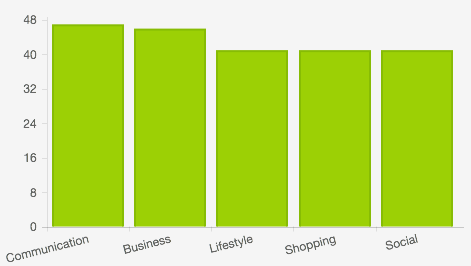
\includegraphics[width=\columnwidth, angle = 0]{images/OverPrivsGenre.png}
\caption{Rates of Over-permissions by Genre}
\label{fig:overPrivsGenre}
\end{figure}



Users are also able to search through our listing of 64,868 Google Play apps. An example search app search and subset of results is shown in Figure~\ref{fig:appSearch_all}. As shown in Figure~\ref{fig:webpagequery}, users may also explore the data by writing their own queries against the dataset right on the webpage.




% Prebuilt .csv reports
%




 \begin{figure}[h]
\centering
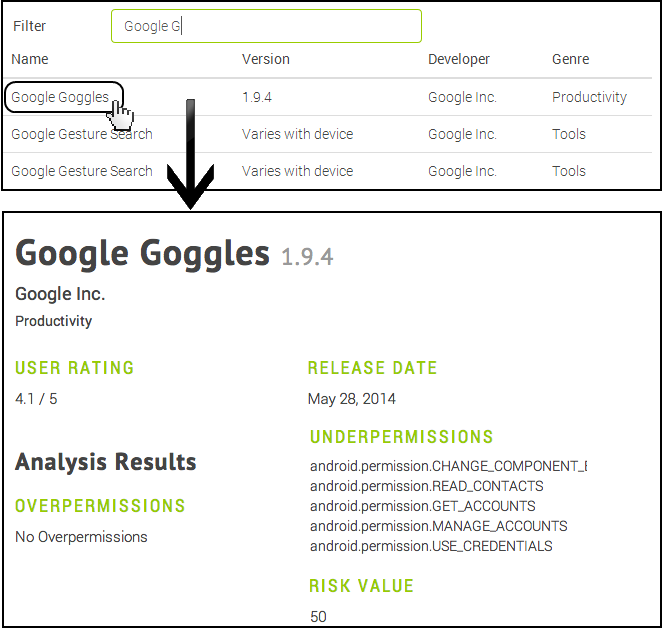
\includegraphics[width=0.98\columnwidth, angle = 0]{images/Google_Googles_ICSE.png}
\caption{Example App Search}
\label{fig:appSearch_all}
\end{figure}



%%% Check to make sure this image looks ok in the print out
% \begin{figure}[h]
%\centering
%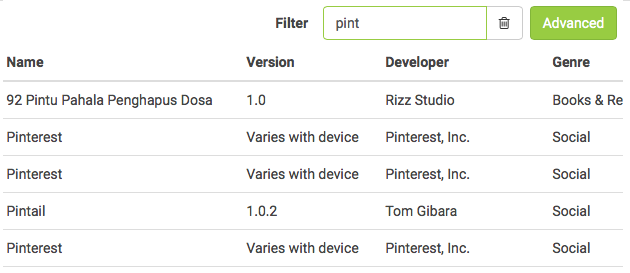
\includegraphics[width=\columnwidth, angle = 0]{images/PinterestSearch_small.png}
%\caption{App Search}
%\label{fig:appSearch}
%\end{figure}
%
%
%%%% Check to make sure this image looks ok in the print out
% \begin{figure}[h]
%\centering
%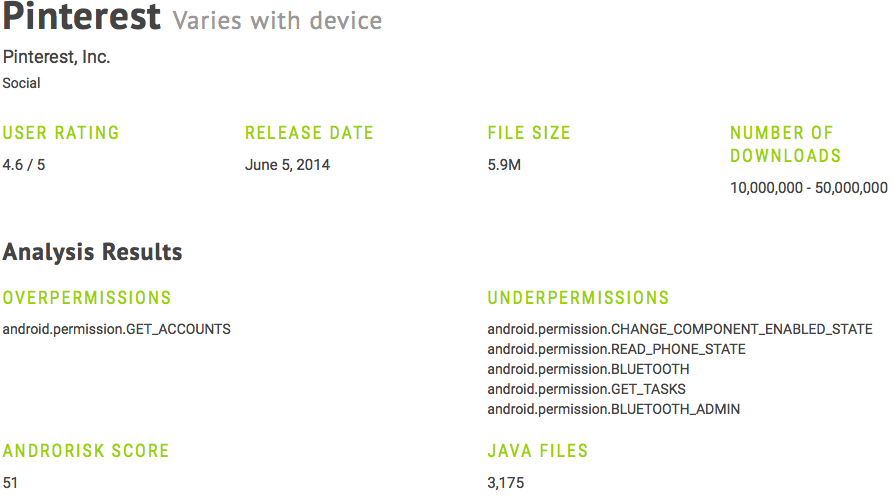
\includegraphics[width=\columnwidth, angle = 0]{images/Pinterest_small.png}
%\caption{Information About Specific App}
%\label{fig:appResults}
%\end{figure}






\begin{figure}[ht!]
\centering
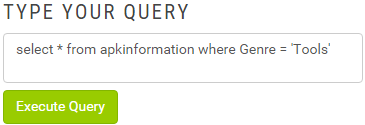
\includegraphics[width=\columnwidth, angle = 0, scale=.8]{images/webpageQuery2.png}
\caption{Webpage Search Query}
\label{fig:webpagequery}
\end{figure}





%
%%%%% Information about signing
%\begin{table}[ht]
%\begin{center}
%\caption{Signing Information}
%\label{Table:SigningInformation}
% \begin{tabular}{ | l | c | } \hline
%
%	  \bfseries Permission & \bfseries   Count \\ \hline
%	
%%	INTERNET &	73,484  \\ \hline
%	
%        	 	
%  \end{tabular}
%\end{center}
%\end{table}





\subsection{Enabled Research}


% Provide Introduction
This dataset provides a wide range of benefits for a Android users, researchers, and app developers. We will next provide several usage scenarios for our provided data.


\textbf{Facilitate research on Google Play apps.} A primary goal of our work is to allow others to extend upon our research. Since we collected a variety of information from Google Play and from static analysis tools, comparisons could be done against the user ratings of the apps and a variety of quality and security-related metrics. Researchers could also analyze apps and how they evolve on a yearly basis, since some of our data dates back to early 2010. Permissions data (we collected 558,216 permissions from Google Play apps alone) could be used to provide insight in numerous ares including the tendencies of permissions use and the popularity of various permissions.


%%% Maybe remove this
%% App versions
%Since our focus was to collect apps using a spread approach and did not target specific apps or versions, we only collected 1,350 apps with three versions, and 303 apps with at least five versions. However, this still provides a crucial dataset of how apps may evolve on a small scale and is especially important since attaining previous versions of apps can be extremely challenging. Future research could be conducted to see how apps evolve with each release in a variety of areas including user ratings, permissions, along with several areas of security and quality metrics.


We collected several forms of signing information about each app which could also prove useful for future researchers. Collecting and validating previous app versions is difficult, and while we are unable to provide the actual .apk file, we are able to provide the signing key --- which may be used to verify the authenticity of other apps. Although developers often use different app and developer names, one way to identify the creator of an app is through the the md5 key. Individual developers may use the same md5 value to sign multiple apps, which is a reliable method of identifying the actual creator of an app. Additionally, we collected  other signing information about the apps including various owner and issuer values and the sha1 and sha256 values.


 \textbf{Facilitate research on Malware.}
 In order to better detect and defend against malware, we need to understand more about it such as how it is created, evolves, and its common characteristics. Including data from both benign and malicious apps will enable researchers to study these apps in a variety of ways including how malware is evolving, signing information, app quality, and requested permissions.




% Permission usage in apps
% Compare different apps against one another
%


%Our data may be easily downloaded by researchers for a variety of tasks.
%
%We collected 558, 216 total requested permissions, which may be used in a variety of areas including checking to see if
%
%
%We also collected 125,129 overprivileges and 228,475 underprivileges.





%\textbf{Benchmark Dataset} Our generated data may be used as a benchmark data set for researchers in evaluated their developed static analysis tools. We believe that our data is unbiased since we were using an array of previously developed tools, and were not attempting to present any tools of our own.


%%% Look at historical versions of apps
%



\section{Limitations \& Future Work}
\label{sec: Limitations}

While we feel that our dataset is robust and quite useful for a variety of reasons and uses, there is room for improvement and future work. Although we analyzed 64,868 apps, there are over 1.4 million~\cite{appbrain_URL} on Google Play alone, (with numerous versions of each of these apps) --- we've only analyzed a very minor portion of all available app candidates. We have also only examined free apps, excluding a significant population (paid apps) in our analysis.

We used a variety of static analysis tools in our analysis, but there are numerous other existing tools which could have been used including Sonar\footnote{\url{http://www.sonarqube.org}}, Permlyzer~\cite{6698893}, and FindBugs{\footnote{\url{http://findbugs.sourceforge.net}}. While no reverse engineering process can ever be considered perfect, our technique has been demonstrated to be highly effective in previous research~\cite{apvrille2012android,chawla2014transfiguring}.

%%% Not sure if I should leave this in
%One of our primary goals was to create a data set which was easily sharable, so we decided to encapsulate all of our data in a sqlite database. Unfortunately, due to the large amount of stored information, this may cause the website to work very slowly. Future work should be done to create a more robust mysql database backend, and then create a component for exporting the data into sqlite format.


%%% All issues are possible issues


% Do not have every version of the apps. The collection process was more of a shotgun approach to gather as much of a wide variety of apps as possible.


% ? Will alter to analyze 'M' apps, but there are presently not many available apps


\section{Conclusion}
\label{sec: conclusion}

We created a valuable, publicly accessible dataset by collecting and analyzing 64,868 apps from Google Play and various malware sources. This dataset is beneficial to developers, researchers, and Android users in not only understanding existing apps, but in how apps are developed, evolve, and are maintained. The collected data is publicly available on the project website: \url{http://darwin.rit.edu}

\balance
\bibliographystyle{abbrv}
\bibliography{DarwinData}

% That's all folks!
\end{document}


% ************************



%%% Todo
% Remove some items on the Address bar
% Use se emails




%todo:
%   XDouble check to make sure that the format is correct
%	Work on the title
%	XCheck to make sure that I am addressing what was said about previous MSR paper
%	Write Queries for posting on website
%	
%	Update all numbers based on the actual tools analyzed. There will need to be some clean up
%	Update .sqlite file with views already in it. Mention these views in the paper & on website.
%	"dataset" not "data set"
%	Say we analyzed app versions, not apps. This means that it might not be a bad idea to change the title.
% 	Probably remove some of the references
%	Create schema for website (might be able to reuse much of what was used for F-Droid) and better FAQ
%	Consistent user of over and under privs
%   ? Should the overall numbers be updated with what is reported in the views?
%   How do SAC reviews impact this paper?
%   Add malware info to website?
%   Analyze the new malware area (Mei) https://github.com/ytisf/theZoo ?
%   Create the views in the malware sqlite files

% Website: http://2016.msrconf.org/#/data

% Thoughts
%	Use the same 'safe' tools as were mentioned in Previous MSR paper to reduce
%	? Should I combine the malware results in here as well?




% Notes:
%	"Google Play" - it is 2 words




